\documentclass[11pt]{article}
\usepackage[landscape,margin=0.55in]{geometry}
\usepackage{graphicx}
\usepackage{booktabs}
\usepackage{amsmath,amssymb}
\usepackage{xcolor}
\usepackage{float}
\providecommand{\FloatBarrier}{}
\usepackage[colorlinks=true,linkcolor=accent,urlcolor=accent]{hyperref}

\graphicspath{{figures_solo/}{figures_local/}{../../references/paper_figures/}}

\definecolor{accent}{RGB}{20,90,150}
\makeatletter
\renewcommand\section{\@startsection{section}{1}{\z@}%
  {-2.6ex \@plus -1ex \@minus -.2ex}{1.2ex \@plus.2ex}%
  {\normalfont\Large\bfseries\color{accent}}}
\renewcommand\subsection{\@startsection{subsection}{2}{\z@}%
  {-2.2ex\@plus -1ex \@minus -.2ex}{0.6ex \@plus .2ex}%
  {\normalfont\large\bfseries\color{accent}}}
\makeatother
\setlength{\parskip}{0.3em}
\setlength{\parindent}{0pt}

% paper | ours pair, large (landscape: each ~4.9 in wide)
\newcommand{\pair}[2]{%
\begin{center}
\begin{minipage}[c]{0.455\textwidth}\centering\includegraphics[width=\textwidth]{#1}\end{minipage}\hfill
\begin{minipage}[c]{0.455\textwidth}\centering\includegraphics[width=\textwidth]{#2}\end{minipage}
\end{center}}
\newcommand{\blurb}[1]{{\small #1}\par}

\begin{document}

% ===================== TITLE =====================
\begin{center}
{\color{accent}\rule{\textwidth}{1.4pt}}\\[0.6em]
{\LARGE\bfseries RS Quark Sector: Literature Reproductions and Custodial\par}
\vspace{0.3em}
{\large Minimal (non-custodial) Randall-Sundrum validated against the published
figures, plus what custodial symmetry changes.\quad June 2026\par}
\vspace{0.2em}
{\color{accent}\rule{\textwidth}{1.4pt}}
\end{center}

\blurb{Everything is the \textbf{anarchic baseline (lane A)}, the literature strawman
used to validate the code. It is \emph{not} production: production as run (lane B,
fit-aligned MFV) is a $\varepsilon_K$ wall near \textbf{7 TeV}, the FPR ideal
(lane C, $V_{5KM}$) near \textbf{2 TeV}. So the $\sim$30 TeV anarchic
$\varepsilon_K$ cloud is the strawman, not ``our floor.''}

% ===================== FLOORS =====================
\section{Floor summary}

\blurb{Two floors. \textbf{Typical} (median anarchic point allowed):
$\sim$30 TeV, set by $\varepsilon_K$. \textbf{Existence} (best fine-tuned point
allowed): $\sim$18--20 TeV, set by $S,T,U$. Flavor is tunable (align
$\mathrm{Im}\,M_{12}\to0$); $S,T,U$ is not, which is why custodial exists.}

\begin{center}
\small
\begin{tabular}{@{}llll@{}}
\toprule
Constraint & Typical (median) & Existence (best/tuned) & Tunable? \\
\midrule
$\varepsilon_K$       & $\sim$30 TeV (lane A; B $\sim$7, C $\sim$2) & $<\!1$ TeV & yes \\
$\Delta m_d,\ \Delta m_s$ & few TeV & $<\!1$ TeV & yes \\
$D^0$, $\Delta m_K$   & low      & $<\!1$--3 TeV & yes \\
$Z\to b\bar b$        & $\sim$5 TeV & $\sim$4.6 TeV & no (gauge; $c_{Q_3}$ set by $m_t$) \\
$S,T,U$               & $\sim$20 TeV & $\sim$18--20 TeV & no (no Yukawa freedom) \\
\midrule
\textbf{Combined}     & \textbf{$\sim$30 TeV} ($\varepsilon_K$) & \textbf{$\sim$18--20 TeV} ($S,T,U$) & \\
\bottomrule
\end{tabular}
\end{center}

\clearpage
% ===================== REPRODUCTIONS =====================
\section{Reproductions (paper left, ours right)}

\blurb{Each is the correctly cropped single minimal / S1 paper panel on the left, our
fixed-code reproduction on the right, in the same axes.}

\subsection{$S,T,U$ oblique \quad{\small (Casagrande et al.\ 0807.4937, Fig.~4)}}
\pair{{casagrande_0807.4937_fig4_ST_solo}.png}{solo_STU.png}
\blurb{The minimal wedge climbs steeply in $T$ (the volume-enhanced $T$ problem) and
leaves the ellipse fast. This irreducible bound sets the $\sim$18--20 TeV existence floor.}

\subsection{$Z\to b\bar b$ couplings \quad{\small (Casagrande et al.\ 0807.4937, Fig.~8)}}
\pair{{casagrande_0807.4937_fig8_gLgR_solo}.png}{solo_Zbb_gLgR.png}
\blurb{The $(g_L^b,g_R^b)$ stripe slides to less-negative $g_L^b$ as $M_{KK}$ drops,
staying near the SM. Gauge-dominated and weak; the bound reaches only $\sim$5 TeV (post-fix).}

\subsection{$\varepsilon_K$, S1 standard \quad{\small (Bauer et al.\ 0912.1625, Fig.~4 top-left)}}
\pair{{bauer_0912.1625_fig4_epsK_solo}.png}{solo_epsK_cloud.png}
\blurb{Anarchic $|\varepsilon_K|$ cloud, $\sim$6 decades (grey = mass+CKM gated;
blue = $Z\to b\bar b$-consistent; orange = in the $|\varepsilon_K|$ window).
\textbf{S1 ``standard'' = independent per-generation RH-down bulk masses}
($c_{d_1},c_{d_2},c_{d_3}$ each fit to masses and CKM, full anarchy). This is the
scenario our production catalog implements. The 95\% quantile enters the band near 10 TeV.}

\subsection{$\varepsilon_K$, S2 aligned \quad{\small (Bauer et al.\ 0912.1625, Fig.~4 top-right)}}
\pair{{bauer_0912.1625_fig4_epsK_S2_solo}.png}{solo_epsK_cloud_S2.png}
\blurb{\textbf{S1 vs S2 is exactly one change.} S2 ``aligned'' imposes a
\emph{common} RH-down bulk mass $c_{d_1}=c_{d_2}=c_{d_3}$ (a $U(3)$ flavor symmetry
on the RH down quarks); everything else (same draws, same gate, same colouring) is
identical. In code the switch is a single flag (\texttt{common\_cd}): both fit the
three RH-down bulk masses to masses and CKM, then S2 averages them to their mean
while S1 keeps them independent. That single alignment suppresses the down-sector
$\Delta F=2$ mixing, so the $\varepsilon_K$ cloud collapses toward the band (floor
$\sim$10 TeV in S1 $\to$ $\sim$2--3 TeV in S2) and the orange in-band fraction
fattens. It is a different model (an extra flavor symmetry), not our scan, and not
custodial.}

\blurb{\textbf{Lowest existence point, S1 and S2.} The lowest $M_{KK}$ at which
\emph{any} point passes $\varepsilon_K$ is below the 1 TeV grid bottom for
\emph{both} scenarios: $\varepsilon_K$ is fully tunable, so even anarchic S1
occasionally throws an accidentally-aligned point (small $\mathrm{Im}\,M_{12}$) that
is consistent at 1 TeV. What S1 $\to$ S2 changes is the \emph{density} of passing
points, not this floor: at $M_{KK}\le3$ TeV, S1 has only $\sim$470 consistent draws
(a fluke), S2 has $\sim$21{,}000 ($\sim$44$\times$ more, the $U(3)$ alignment makes
consistency generic). So alignment lowers the \emph{typical} floor ($\sim$10 to
$\sim$2--3 TeV), not the existence floor ($<$1 TeV for both).}

\subsection{Consistency fraction, S1 \quad{\small (Bauer et al.\ 0912.1625, Fig.~5)}}
\pair{{bauer_0912.1625_fig5_consistency_solo}.png}{solo_consistency.png}
\blurb{Fraction of \textbf{S1} (standard) anarchic points consistent with
$|\varepsilon_K|$ vs $M_{KK}$, the black solid curve in Bauer's Fig.~5; the
$1/M_{KK}^2$ decoupling matches the paper.}

\subsection{$\Delta F=2$ amplitudes, S1 \quad{\small (Blanke et al.\ 0809.1073, Fig.~2)}}
\pair{{blanke_0809.1073_fig2_M12planes_solo}.png}{solo_ReIm_M12.png}
\blurb{Re vs Im of the KK contribution to $M_{12}$ for $K$ and $B_s$ (\textbf{S1}
ensemble). For kaons the imaginary part dominates the real part by $\sim$100$\times$;
ours is 106$\times$.}

\clearpage
% ===================== CUSTODIAL =====================
\section{Custodial symmetry: what it changes}

\blurb{Custodial RS ($\mathrm{SU(2)}_L\times\mathrm{SU(2)}_R\times\mathrm{U(1)}_X
\times P_{LR}$) is an \textbf{electroweak} cure. $\mathrm{SU(2)}_R$ protects the
oblique $T$; the discrete $P_{LR}$ protects the $Z b_L$ vertex. It does
\textbf{nothing} to $\varepsilon_K$, because that is set by the color-octet KK-gluon
$C_4$, an electroweak singlet. Only flavor alignment moves the $\varepsilon_K$ wall.
The two protections are separable (oblique floor vs PDG-2025 $U$-fixed ellipse;
$\delta g_L^b$ at $M_{KK}=3$ TeV):}

\begin{center}
\small
\begin{tabular}{@{}lll@{}}
\toprule
EW model & oblique $S,T,U$ floor & $Z b_L$ shift $\delta g_L^b$ \\
\midrule
minimal RS               & 16.0 TeV ($T$ problem)      & $2.6\times10^{-3}$ (unprotected) \\
$\mathrm{SU(2)}_R$ only   & 5.8 TeV ($T$ fixed; set by $S$) & $2.6\times10^{-3}$ (= minimal) \\
$\mathrm{SU(2)}_R+P_{LR}$ & 5.8 TeV (unchanged)        & $0$ (protected) \\
\bottomrule
\end{tabular}
\end{center}
\blurb{$\mathrm{SU(2)}_R$ does the whole oblique job ($16\to5.8$ TeV); $P_{LR}$
collapses $\delta g_L^b$ without touching the oblique floor. Independent cures.}

\subsection{$S,T,U$ with custodial \quad{\small (CGHNP 0807.4937, Fig.~4 right panel $|$ ours)}}
\pair{paper_ST_custodial.png}{ours_ST_custodial.png}
\blurb{The custodial $T$ collapses to $\approx0$ (the volume-enhanced $T$ is gone);
the residual floor is the \emph{unprotected} $S$. Left is the literal right half of
the same Fig.~4 whose left (minimal) half is the $S,T,U$ reproduction above.}

\subsection{$Z\to b\bar b$ with $P_{LR}$}
\begin{center}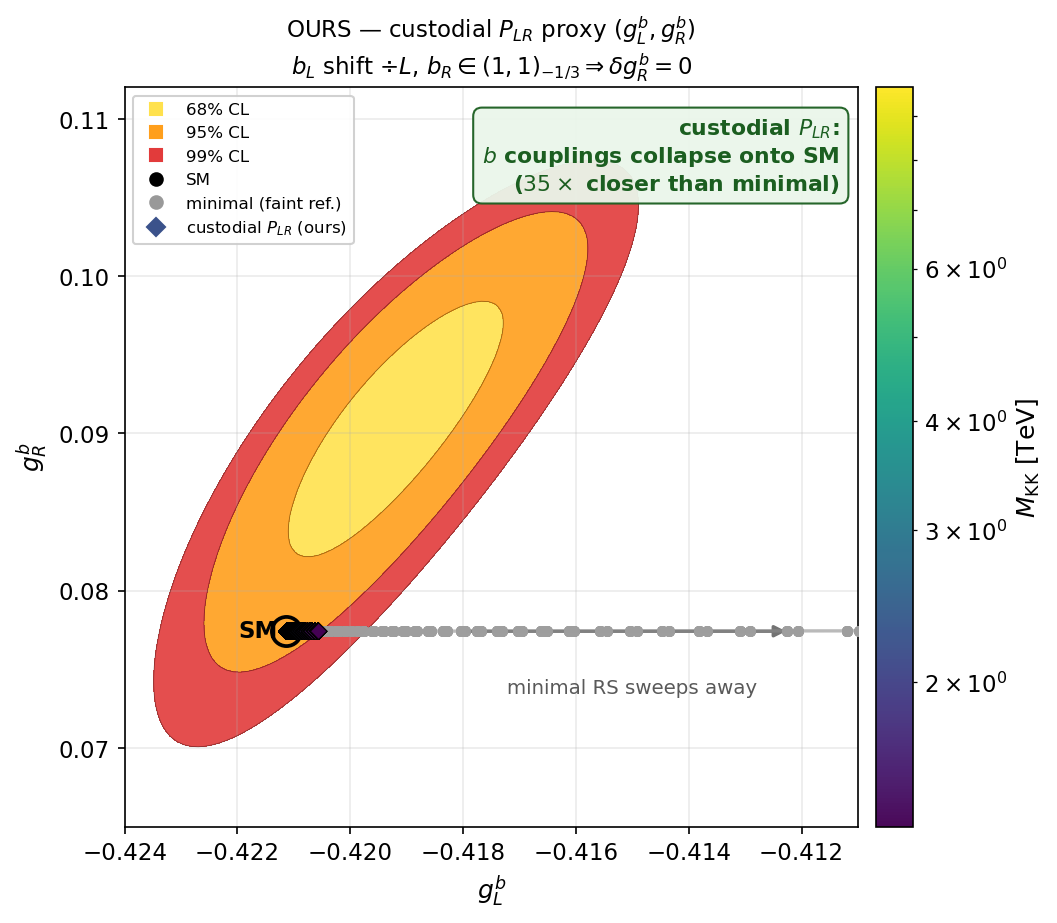
\includegraphics[width=0.56\textwidth]{ours_Zbb_custodial.png}\end{center}
\blurb{$P_{LR}$ collapses the $b$ couplings onto the SM ($\delta g_L^b$ suppressed by
$1/L$, $\delta g_R^b\to0$ for $b_R\in(1,1)_{-1/3}$), $\sim$35$\times$ closer than the
minimal stripe, which sweeps away. No published $(g_L^b,g_R^b)$ custodial panel exists
to compare against.}

\subsection{$\varepsilon_K$ with custodial: unchanged}
\blurb{Custodial is blind to $\varepsilon_K$: the cloud is identical to the S1 panel
above, because the binding operator is the color-octet, EW-singlet KK gluon. Blanke
0809.1073 computes the full $\Delta F=2$ inside the custodial model and still finds
$M_{KK}\gtrsim18$--30 TeV. Custodial is an electroweak cure, not a flavor cure.}

\end{document}
